\chapter{Materiales}
\section{Parkinson's Progression Markers Initiative (PPMI)} 
\begin{figure}[h]
	\centering
	
\includegraphics[width=0.3\textwidth]{imagenes/ppmi logo.PNG}
	\caption{Logo de la PPMI}
	\label{fig:ppmi}
\end{figure}

La PPMI es un estudio clínico que consiste en el seguimiento de un conjunto de individuos. Su objetivo es facilitar la investigación basada en la búsqueda de identificadores de la progresión de la enfermedad de Parkinson (EP), ya que para poder obtener tratamientos más efectivos es fundamental la detección temprana de marcadores específicos de la enfermedad y comprender su progresión. \cite{HomePark57:online}\\

Este proyecto fue lanzado en el 2010 con la colaboración de investigadores, pacientes y la Michael J. Fox Foundation (MJFF). Entre los pacientes incluidos se encuentran tanto individuos recién diagnosticados de EP, identificados dentro del grupo PD, como sujetos que no la padecen pero que tienen riesgo de de desarrollarla en el futuro, los cuales entran dentro del grupo de control HC, formado por 196 individuos.\\

Dentro del grupo de pacientes que han sido diagnosticados con Parkinson, hay tres subgrupos dentro de los cuales han sido clasificados en función del nivel de desarrollo del declive cognitivo:
\begin{itemize}
	\item PD-CU: Individuos que no presentan deterioro cognitivo. Esta compuesto por un total de 323 pacientes.
	\item PD-MCI: Individuos a los que se les ha detectado un declive cognitivo leve, siendo en total 83 pacientes.
	\item PDD: Individuos diagnosticados con demencia, son un total de 17 sujetos. 
\end{itemize}

Cada uno de los participantes permanece en el estudio durante varios años, permitiendo un seguimiento durante este tiempo en el que se toman medidas de distintos parámetros fundamentales para estudiar la progresión de la enfermedad: marcadores biológicos, evaluaciones clínicas, pruebas de imágenes cerebrales o análisis de líquido cefalorraquídeo. \cite{marek2011parkinson}\\
 
La PPMI permite que la búsqueda de biomarcadores sea más rápida y eficaz, ya que permite la colaboración entre diferentes científicos y el entendimiento de los cambios en el curso clínico entre unos pacientes u otros.


\section{Leaspy}
\label{sec:leaspy}
\begin{figure}[h]
	\centering
	
\includegraphics[width=0.3\textwidth]{imagenes/leaspyLogo.PNG}
	\caption{Logo de Leaspy}
	\label{fig:leaspy}
\end{figure}
Para el análisis de datos con estructura espacial con el objetivo de estimar el
avance de enfermedades, así como para el estudio de datos longitudinales se
desarrollaron las siguientes herramientas de software: Leasp para C++ y Leaspy
para Python. El segundo es utilizado mayoritariamente para estimar la progresión
de enfermedades a largo plazo, imputar valores faltantes y la simulación de
cohortes virtuales.

\subsection{Leasp: Paquete de C++ para el Análisis de Datos Longitudinales
	Estructurados Espacialmente}

Este paquete trabaja con datos obtenidos tras la observación de pacientes a lo
largo del tiempo. Su función se basa en: reconstruir la trayectoria a largo
plazo de los pacientes a partir de las observaciones, ubicar cada medida de cada
paciente en relación con la linea de tiempo promedio grupal y medir el efecto de
ciertos cofactores como por ejemplo el género en el transcurso de la señal. \cite{Welcomet75:online}\\

Esta herramienta puede trabajar tanto con variables escalares, como puntuaciones
clínicas o evaluaciones cognitivas; como con 	datos de red (PET SUVR).\\

El diseño de Leasp se centra en la interacción entre un algoritmo y un modelo
basado en entradas escalares y de red. Con esta biblioteca se tiene acceso a
distintas carpetas que permite el uso de varias funcionalidades:
\begin{itemize}
	\item Aplicación de procedimientos matemáticos
	\begin{itemize}
		\item Calibración
		\item Personalización
		\item Simulación
	\end{itemize}
	\item Funciones de procesamiento
	\item Herramientas de visualización
\end{itemize}

Para su correcta utilización a continuación se muestran algunas instrucciones y
pasos que se deben seguir:

\begin{description}
	\item {\textbf{Requisitos.}} Es necesario instalar las siguientes bibliotecas:
	\textit{tinyxml} (lectura y preprocesamiento de archivos xml),
	\textit{googletest} (pruebas de unidad y funcional ) y  \textit{Armadillo} (uso
	de algebra lineal para vectores y matrices) 
	
	\item {\textbf{Instalación.}} Desde la terminal, ejecutar los comandos que se
	muestran a continuación:
	\begin{enumerate}
		\item \texttt{git clone https://gitlab.com/icm-institute/aramislab/leasp}
		\item \texttt{git submodule init}
		\item \texttt{git submodule update}
		\item \texttt{. mkdir build \&\& cd build}
		\item \texttt{. cmake --options}
		\item \texttt{. make --options\}}
	\end{enumerate}
	
	\item {\textbf{Ejecución del software.}} Agregación del software a
	\texttt{/protect/T1/textdollarPATH} y ejecucion del siguiente comando:
	\begin{center}
		\texttt{leasp fit model\_stgs.xml algorithm\_stgs.xml data\_stgs.xml sampler\_stgs.xml}
	\end{center}
	
	\begin{itemize}
		\item \texttt{fit}: Ajuste de la curva promedia grupal a medidas individuales.
		\item \texttt{model\_settings}: Da información de los parámetros y del tipo de modelo	que se va a ejecutar.
		\item \texttt{algorithm\_settings.xml}: Define parámetros del algoritmo como el numero total de iteraciones.
		\item \texttt{data\_settings.xml}: Recopila la ruta de los archivos de datos.
		\item \texttt{sampler\_settings.xml}: Enumera las muestras utilizadas en el procedimiento de estimación, junto con sus parámetros.
	\end{itemize}
	
	\item {\textbf{Salidas de la estimación.}} Se producen tres archivos en el proceso: \\
	\texttt{convergence\_parameters.csv} muestra la convergencia del modelo.\\ \texttt{population\_parameters.csv} define parametros para el promedio grupal a largo plazo.\\ \texttt{individual\_parameters.csv} que son parametros temporales y espaciales para la trayectoria individual.
\end{description}

\subsection{Leaspy: Toolbox de Python para Aprender Patrones Espaciotemporales de la Progresión de la Enfermedad} \label{sec:parámetros de leaspy}

Para el estudio de datos longitudinales y ver la progresión de enfermedades a largo plazo en Python se desarrollo la herramienta Leaspy. Basándose en el modelo de efectos mixtos, permite la reconstrucción de la evolución promedia e individual. Además, permite abordar problemas de los estudios de datos longitudinales, como el que cada paciente tenga un numero de observaciones distinto, permite trabajar con valores faltantes y medidas de datos estructurados espacialmente (imágenes o redes), gracias a la geometría de Riemann. También es de gran utilidad trabajando con medidas en un periodo de tiempo corto, cuando el fenómeno de estudio es de larga duración. Otras aplicaciones permiten predecir puntos temporales futuros y simular nuevas cohortes a partir de los parámetros obtenidos de un ya existente. La calidad del paquete se garantiza mediante pruebas unitarias, control de versiones git e integración continua.
\begin{figure}[h]
	\centering
	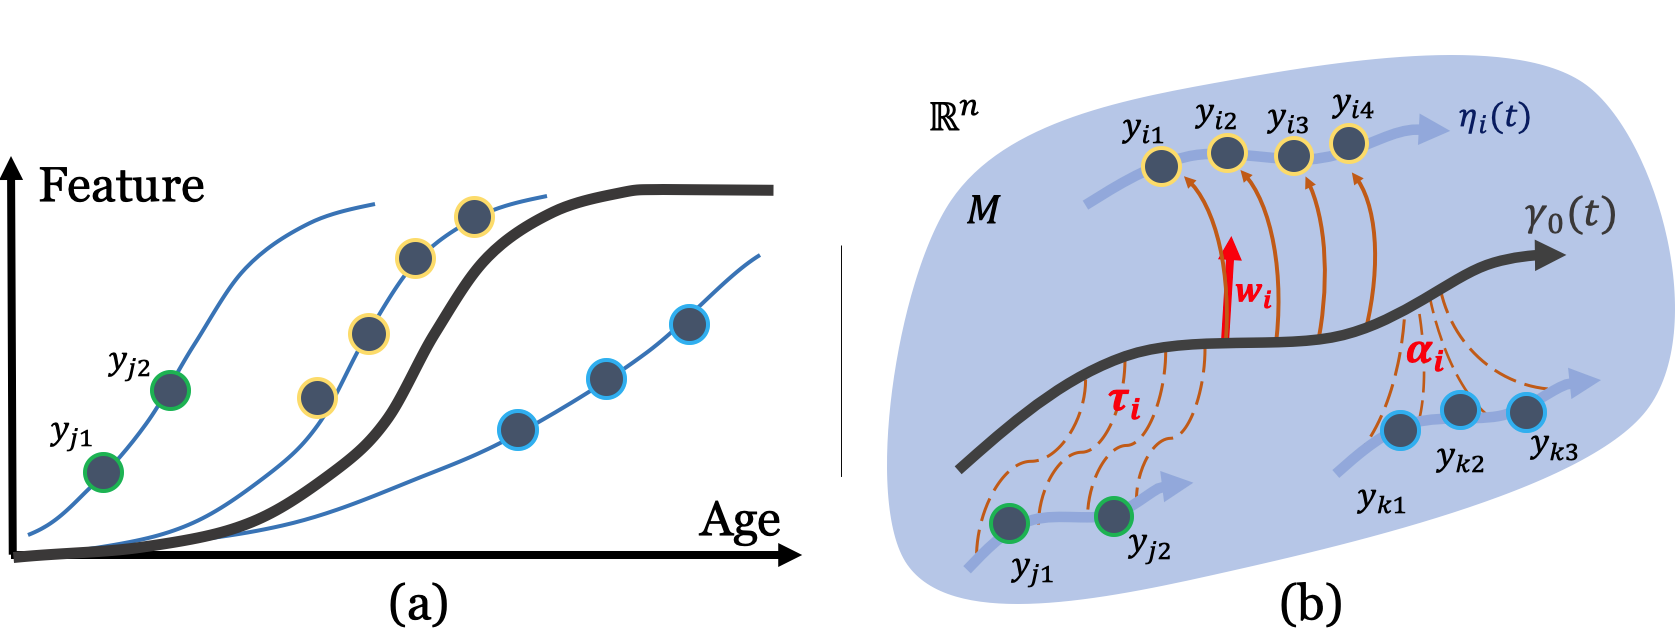
\includegraphics[width=0.9\textwidth]{imagenes/leaspy_trayectories.PNG}
	\caption{Curvas características de la progresión de los marcadores.}
	\label{fig:trayectories}
\end{figure}

El siguiente modelo, basado en efectos mixtos, representa un conjunto de datos longitudinales $y=(y_{ij},t_{ij})\ 1 \leq i \le n, 1 \le j \le k_{i}$ de $\textit{n}$ pacientes. El número de observaciones de cada individuo $i$ se representa con $k_{i}$, siendo los tiempos de cada observación $t_{i1} < ... < t_{ik_{i}}$.

\begin{equation}
	y_{ij} = f(\theta_{geom}, z_{i}, t_{ij} ) + \epsilon_{ij}
\end{equation}

$\theta_{geom}$ son los parámetros del modelo, $z_{i}$ es la variación de cada individuo respecto a la trayectoria promedio grupal y $\epsilon_{ij}$ es un ruido gaussiano. El objetivo es calcular los parámetros anteriores que hagan que los datos sean lo más verosímiles posibles. Con Leaspy se pueden realizar los siguientes procedimientos:

\begin{enumerate}
	\item Calibración: consiste en estimar $y$ a partir de $\theta$, obteniendo la curva promedio del grupo a largo plazo. Esta basada en el algoritmo MCMC-SAEM y la varianza adaptativa y el descenso de gradiente mejoran la velocidad de convergencia.
	\item Personalización: Teniendo $\hat{\theta}$, se reconstruyen las trayectorias individuales obteniendo la variable oculta $z_{i}^{*}$. Este procedimiento estadístico incluye métodos Powell y L-BFGS.
	\item Reconstrucción, imputación de valores faltantes y predicción: Con las variables resultantes de los dos pasos anteriores, se calcula $y_{ij}^{*}=f(\hat{\theta}, z_{i}^{*}, t_{ij})$ para distintos periodos de tiempo.
	\item Simulación: Se genera un individuo completamente nuevo ($z_{i}^{0}$) a partir de $\hat{\theta}$ y un conjunto de variables individuales, pudiendo repetir el proceso hasta conseguir una cohorte virtual. Este método está basado en estimaciones condicionales gaussianas multivariadas y en funciones de densidad kernel.	
\end{enumerate}

La programación en Python de los cuatro procesos anteriores sigue una metodología bastante amigable para le usuario, ya que menos para la reconstrucción, el resto se estructuran de la siguiente manera:
\begin{itemize}
	\item \textbf{Definición de parámetros:} el objeto \texttt{AlgorithmSettings} se encarga de esta función. En su llamada se fija el algoritmo que se quiere utilizar y otras variables. También se pueden cargar a través de kwargs o archivos json.
	\item \textbf{Llamada a las funciones:} tras el paso anterior, se realiza la llamada al método que se este llevando a cabo, introduciendo los parámetros definidos: \texttt{leaspy.fit(...)} para la calibración, \texttt{leaspy.personalize(...)} para personalizar el modelo, \texttt{leaspy.reconstruct(...)} para reconstruirlo y\\\texttt{leaspy.simulate(...)} para realizar una simulación.
	\item \textbf{Visualización y registro:} Leaspy también permite guardar archivos de registro y otras variables en archivos csv y json, lo que también permite volver a cargarlos en el programa; y se pueden visualizar perfiles de progresión o reconstrucciones de trayectorias.
\end{itemize}

Además, para comprender el funcionamiento de este entorno, hay que tener claros los parámetros con los que trabaja Leaspy a la hora de obtener los modelos \cite{DiseaseC47:online}. Por una parte, a la hora de estimar la trayectoria de la progresión media de un biomarcador se utilizan los parámetros \textit{'long-term'}:
\begin{itemize}
	\item $\mathbf{t_{k}}$: Edad para la cual se obtienen los parámetros  que definen la curva general (p0 y u0).
	\item $\mathbf{p_{k}}$: Indica el valor normalizado de la variable en el tiempo t0 para la trayectoria a largo plazo.
	\begin{equation}
		p_{k}=\gamma_{k}(t_{k})
	\end{equation}
	\item $\mathbf{u_{k}}$: Representa la velocidad de aumento del valor de dicha variable en función del tiempo.
	\begin{equation}
		u_{k}=\frac{d}{dt}(\gamma_{k}(t_{k}))
	\end{equation}
\end{itemize}
Estás variables permiten estimar la trayectoria global media de cada biomarcador ($\gamma_{k}$). Esto se realiza con la función \textbf{leaspy.fit}, la cual toma las medidas longitudinales de los sujetos de la base de datos y obtiene los parámetros que definen la curva \textit{'long-term'}. Una vez obtemidos los parámetros, la curva se obtiene con la siguiente ecuación:
\begin{equation}
	\gamma_{k}=\frac{1}{1+((\frac{1}{p_{k}}-1)*exp(-\frac{u_{k}*(t-t_{0})}{p_{k}*(1-p_{k})}))}
\end{equation}

\begin{figure}[h]
	\centering
	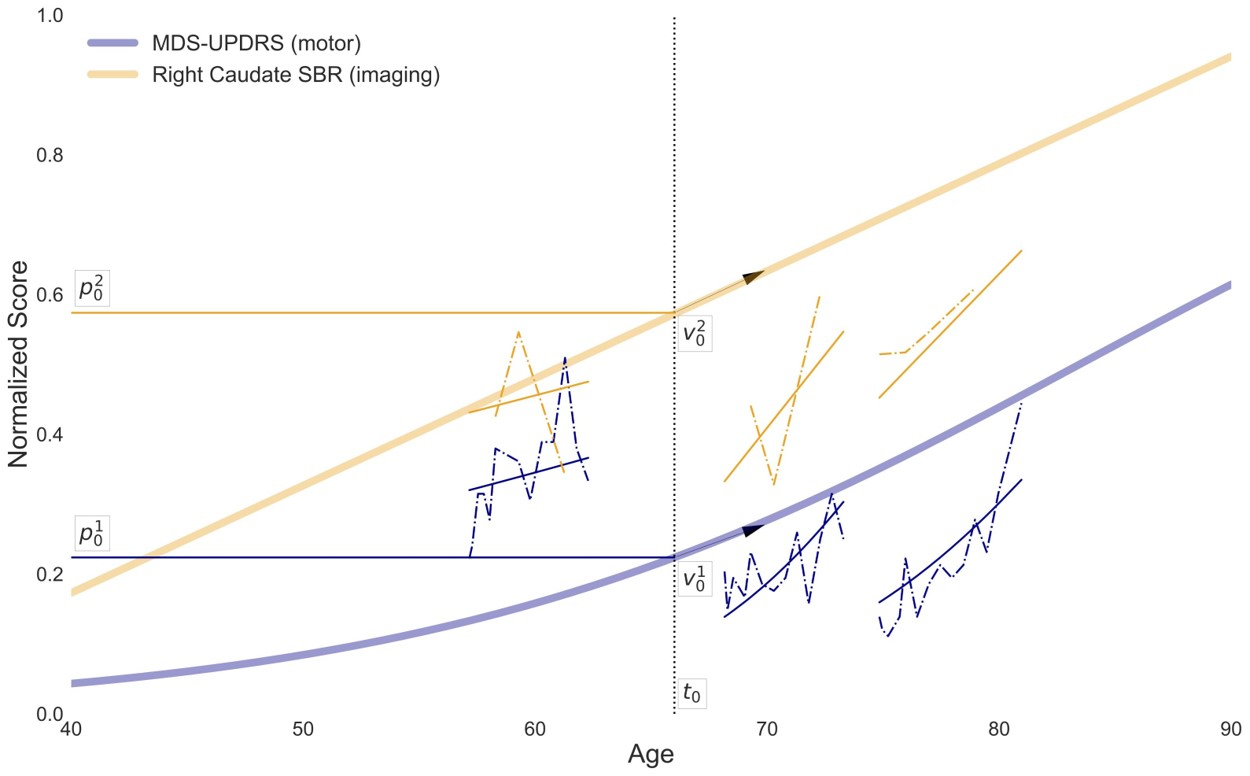
\includegraphics[width=0.85\textwidth]{imagenes/PARÁMETROS LONG TERM.JPG}
	\caption{Representación de los parámetros de una trayectoria long-term}
	\label{fig:long-term}
\end{figure}

Una vez conseguido esto, Leaspy utiliza la función \textbf{leaspy.personalize} para obtener los parámetros \textit{'short-term'}:
\begin{itemize}
	\item $\mathbf{\tau_{i}}$: Representa la reserva cognitiva en años, es decir, el tiempo del que dispone un sujeto antes de alcanzar el declive cognitivo. un valor mayor que 0 indica que la progresión de la enfermedad es más tardía que la media, en cambio un valor negativo indica que que es más temprana.
	\item $\mathbf{\alpha_{i}}$: EL factor de aceleración marca si en el caso del sujeto seleccionado, la enfermedad avanza a mayor velocidad que la media ($\alpha_{i}>1$) o a menos velocidad ($\alpha_{i}<1$).
	\item $\mathbf{w_{ik}}$: El espacio entre marcadores intermedios  indica la secuencia de eventos descrita por el vector $\tau$, que desplaza cada curva logística, propia del paciente.
\end{itemize}
Estas variables representan la curva característica para un nuevo individuo a partir de la trayectoria general obtenida de un grupo de pacientes facilitado. Esta curva se obtiene con la siguiente ecuación en función de los parámetros \textit{'short-term'}:
\begin{equation}
	\eta_k = \frac{1}{1 + \left( \left( \frac{1}{pk} - 1 \right) \cdot e^{-\frac{(w_{ik} + (u_k \cdot \alpha_i \cdot (t_{ij} - t_0 - \tau_i)))}{pk \cdot (1 - pk)}} \right)}
\end{equation}

\begin{figure}[h]
	\centering
	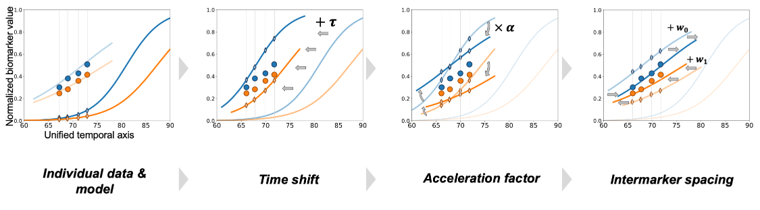
\includegraphics[width=1\textwidth]{imagenes/PARAMETROS SHORT TERM.PNG}
	\caption{Parámetros short-term para la obtención de la curva caracteristica de un nuevo sujeto.}
	\label{fig:short-term}
\end{figure}
Con todas estas herramientas, Leaspy es un entorno versátil y de fácil acceso que permite introducirse en el mundo del análisis y la interpretación de datos longitudinales a través de Python. Permite abordar tareas estadísticas gracias a los modelos y algoritmos en los que esta basado , pudiendo estimara parámetros y simular datos. Además es accesibles desde distintos sistemas operativos como Windows o Linux.

\section{Spyder}
\begin{figure}[h]
	\centering
	
\includegraphics[width=0.3\textwidth]{imagenes/logo_spyder.PNG}
	\caption{Logo de Spyder.}
	\label{fig:spyder}
\end{figure}

"The Scientific Python Development Environment", por sus siglas en inglés Spyder (cuyo logo se ve en la figura \ref{fig:spyder}), es un entorno de desarrollo integrado (IDE) escrito en Python y para Python. Es una herramienta que permite el manejo avanzado de datos, su investigación, análisis, inspección y depuración entre otras muchas acciones. \cite{IPythonC75:online} \\

Esta interfaz consta de varios componentes: 
\begin{itemize}
	\item Editor multi-lenguaje: permite generar, modificar y visualizar código en Python. Además, consta de diversas herramientas y características que facilitan su uso y dan una mayor eficiencia.
	\item \textit{IPython Console}: En este panel se pueden ejecutar comandos, se interactúa con la información y se puede \textit{ejecutar} el código por líneas, celdas o ficheros y depurar el mismo.
	\item Explorador de variables, gráficos y ayuda: En el último panel se pueden escoger distintas ventanas donde observar las variables y parámetros con los que trabaja el programa, buscar ayuda sobre distintos comandos, observar gráficos y navegar por los distintos ficheros del sistema y abrirlos directamente en el entorno.
\end{itemize}

Para este proyecto, se incluyeron varias librerías clave para la programación en este lenguaje y otras con funciones más concretas que simplificaron el desarrollo de ciertos fragmentos. Entre las más importantes se encuentran:
\begin{itemize}
	\item \textbf{NumPy}: creada concretamente para cálculo y análisis de grandes cantidades de datos. Permite trabajar con \textit{arrays} en vez de con listas de Python, lo que otorga un mayor rendimiento.
	\item \textbf{Pandas}: mejora la manipulación y el análisis de datos, integrando el tipo de datos Dataframe, manejo de datos faltantes, reestructuración y segmentación de conjuntos entre muchas otras funciones.
	\item \textbf{Matplotlib}: esta libreria es especifica para la realización de gráficos y visualización de datos. Concretamente se trabajó con el módulo \textbf{Matplotlib.pyplot}, que proporciona una interfaz de porogramación sencilla y con una interfaz gráfica muy similar a la de MATLAB.
	\item \textbf{SciPy}: incluye módulos para realizar cálculos estadísticos, optimización, integración, algebra linear, etc. Es útil para trabajar numericamente con \textit{NumPy arrays}.
	\item \textbf{Seaborn}:Crea gráficos estadísticos extendiendo y simplificando las capacidades de \textit{Matplotlib} y trabajando con estructuras de datos de \textit{pandas}.
	\item \textbf{Os}: permite interactuar con el sistema operativo. Con ella se pueden crear, eliminar y mover archivos y directorios. En este trabajo se utilizó concretamente para guardar y cargar variables en el directorio de trabajo.
	\item \textbf{Leaspy}: es un paquete de software fundamental para este proyecto, explicado en profundidad en el apartado \ref{sec:leaspy}. Utilizado para el análisis de datos médicos longitudinales.
\end{itemize}

Para acceder a este entorno se utilizó la interfaz gráfica de usuario llamada \textit{Anaconda Navigator}. Con ella, además de acceder a \textit{Spyder}  están disponibles muchos otros entornos.


\section{MATLAB}
\begin{figure}[h]
	\centering
	
\includegraphics[width=0.3\textwidth]{imagenes/matlab.PNG}
	\caption{Logo de MatLab.}
	\label{fig:matlab}
\end{figure}

MATLAB es un entorno de programación de alto nivel utilizado para el análisis de datos y cálculos numéricos, desarrollo de algoritmos y visualización de gráficos. \\

Para este proyecto, fue fundamental a la hora de visualizar distintas problemáticas desarrolladas previamente por otros investigadores. Por ejemplo, uno de los objetivos fundamentales es observar la capacidad de predicción de Leaspy en comparación con la precisión de predicción del método RPDPM (Robust Parametric Disease Progression Modeling). Para ello, se utilizó MATLAB como plataforma para observar el funcionamiento de algortimos desarrollados mediante RPDPM.
  
  
\section{PuTTY}
\begin{figure}[h]
	\centering
	
\includegraphics[width=0.2\textwidth]{imagenes/putty.PNG}
	\caption{Logo de PuTTy.}
	\label{fig:putty}
\end{figure}

PuTTy (cuyo logo se ve en la figura \ref{fig:putty}) es una herramienta utilizada para la conexión a servidores y dispositivos remotos para sistemas operativos como Windows \cite{Download87:online}.Es un cliente de terminal bastante flexible que puede utlizar distintos protocolos para realizar la conexión: SSH, Telnet, rlogin entre otros.\\ 

Para este proyecto, se usó esta herramienta para conectarse de forma segura a las máquinas Linux de supercomputación  llamadas \textit{Curie} y \textit{Magerit}, disponibles en la Universidad Politécnica de Madrid. Son destinadas para la ejecución de cargas de trabajo científico que necesitan cómputo intensivo. Para acceder a ellas de forma remota desde Putty, se utiliza el protocollo SSH (Secure SHell) el cual permite entrar de forma segura mediante un canal con la información cifrada \cite{lucas2018ssh}. Para ello, solo hay que introducir en la interfaz de este software \ref{fig:interfaz_putty} la dirección IP y el puerto de la máquina a la que quieres acceder y, posteriormente, el usuario y la contraseña en la propia terminal.\\

\begin{figure}[h]
	\centering
	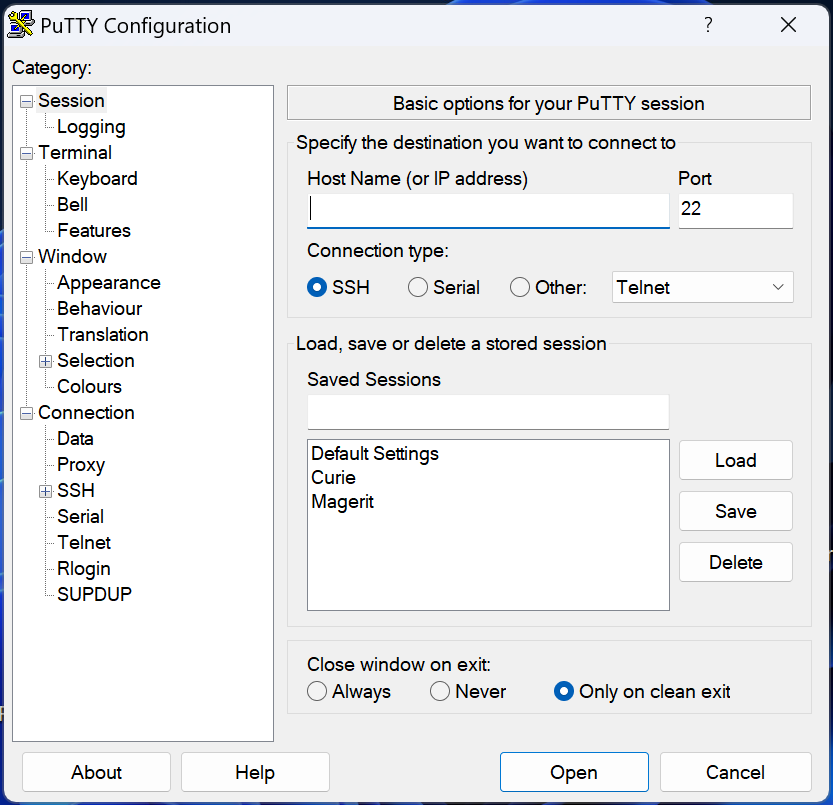
\includegraphics[width=0.5\textwidth]{imagenes/interfaz_putty.PNG}
	\caption{Interfaz de PuTTy.}
	\label{fig:interfaz_putty}
\end{figure}


\section{Xming}
\begin{figure}[h]
	\centering
	
\includegraphics[width=0.3\textwidth]{imagenes/xming.PNG}
	\caption{Logo de Xming.}
	\label{fig:xming}
\end{figure}

Xming es un servidor X para Windows que facilita el uso de aplicaciones gráficas Unix en un entorno Windows \cite{XmingXSe60:online}. Es decir, permite visualizar aplicaciones gráficas que se estén ejecutando en un servidor remoto, al cual en este casos e accede mediante SSH, mostrando las ventanas en el escritorio de Windows.\\

Para su correcto funcionamiento, lo habitual es que una vez está instalado en el dispositivo, cuando se quiera usar deberá dejarse iniciado como un servidor en segundo plano, así más adelante se pueden conectar aplicaciones gráficas desde el cliente SSH, dando acceso a software que no tiene una versión nativa para Windows.\\

Para comprobar el correcto funcionamiento de Xming, una vez lo veas abierto en segundo plano en los iconos ocultos, en la terminal de Putty se debe ejecutar el comando $\mathtt{xeyes\; \&}$ y aparecerá una ventana gráfica con unos ojos, indicando que el software se ha abierto correctamente.


\section{FileZilla Client}
\begin{figure}[h]
	\centering
	
\includegraphics[width=0.2\textwidth]{imagenes/filezilla.PNG}
	\caption{Logo de Filezilla.}
	\label{fig:filezilla}
\end{figure}

A la hora de transferir los archivos del programa desarrollado desde el directorio local al escritorio remoto para poder ejecutarlo desde las máquinas de supercomputación \textit{Curie} y \textit{Magerit}, se utilizó Filezilla Client. Esta herramienta es un cliente de FTP (Protocolo de Transferencia de Archivos) de código abierto, que se utiliza para transferir archivos de un cliente a un servidor \cite{FileZill81:online}.\\

Filezilla consta tanto con el servicio de cliente como con el de servidor, pero son descargados por separado. Desde \textit{Filezilla Client} debe concretarse la dirección del servidor al que desea conectarse para el intercambio de archivos, el usuario y la contraseña del mismo. Para este caso, se utiliza el protocolo FTP, pero \textit{Filezilla} soporta otros como el SFTP (SSH Protocolo de Transferencia de Archivos) o el FTPS (FTP Seguro), que realizan transferencias más seguras.

\section{Curie y Magerit-3}
A la hora de realizar la paralelización del código, para poder estimar el mayor número de modelos posibles de la forma más eficiente y así luego compararlos, se accedió a dos máquina de supercomputación facilitadas por la Universidad Politécnica de Madrid (UPM) y por el Centro de Supercomputación y Visualización de Madrid (CeSViMa), llamadas \textit{Curie} y \textit{Magerit}. \\

Para acceder a las mismas se utiliza la interfaz de Putty como ya se explicó anteriormente. Una vez abierta la terminal, para trabajar con Curie se utiliza la aplicación \textit{Tmux}, un multiplexor de terminales basado en sesiones. Esto permite paralelizar el programa con alto coste de computación y ejecutarlo dentro de las sesiones creadas. Ademas, permite que las distintas tareas sigan ejecutándose aunque se desconecte la sesión. \\

Por otro lado, Magerit es una infraestructura de cómputo posicionada como uno de los supercomputadores energéticamente más eficientes del mundo. Está formado por 72 nodos de propósito general \textit{ThinkSystem} SD530 con procesadores Intel Xeon Gold 6230 y 192 GiB de RAM, y 48 nodos \textit{ThinkSystem} SD530, cada uno de ellos equipado con procesadores Intel Xeon Gold 6240R y 768 GiB de RAM \cite{Descripc17:online}. En este entorno, las tareas se ejecutan mediante ficheros BASH utilizando el comando sbatch.


\section{LaTeX}
\begin{figure}[h]
	\centering
	
\includegraphics[width=0.2\textwidth]{imagenes/latex.PNG}
	\caption{Logo de LaTeX.}
	\label{fig:latex}
\end{figure}

Para la redacción del documento presente se hizo uso de la herramienta LaTeX. Es un sistema de composición de textos de alta calidad importante para generar informes científicos, técnicos y académicos \cite{LaTeXAdo12:online}.